%% grundlagen.tex
%% $Id: grundlagen.tex 28 2007-01-18 16:31:32Z bless $
%%

\chapter{Grundlagen}
\label{ch:Grundlagen}
%% ==============================

%% ==============================
\section{Kryptographie mit öffentlichen Schlüsseln}
%% ==============================
\label{ch:Grundlagen:sec:PublicKeyCrypto}

\subsection{Prinzip}
\label{ch:Grundlagen:sec:PublicKeyCrypto:subsec:Prinzip}

Klassische Kryptographie basiert auf einem \emph{Geheimnis} oder
\emph{privaten Schl\"ussel}, der beiden Kommunikationspartnern bekannt
ist. 

\subsection{Authentisierung von Schlüsseln}
\label{ch:Grundlagen:sec:PublicKeyCrypto:subsec:KeyAuth}

Zweck von PKI oder Web of Trust ist es, die Authentizit\"at der
Bindung von Schl\"ussel/Zertifikat und Identit\"at zu etablieren. Und
das eben auch dann, wenn man selbst diese Bindung nicht \"uberpr\"ufen
kann.

\subsubsection{Zentrale PKI}
\label{ch:Grundlagen:sec:PublicKeyCrypto:subsec:KeyAuth:subsubsec:PKI}

zentral im Sinne von: Es muss einer einzigen zentralen
Authorit\"at/Instanz vertraut werden.

\subsubsection{Web of Trust}
\label{ch:Grundlagen:sec:PublicKeyCrypto:subsec:KeyAuth:subsubsec:WOT}

Zu beachten ist, dass im Rest dieser Arbeit der Begriff
``Schl\"ussel'' ausschliesslich im Sinne des \"offentlichen Teils
eines Schl\"usselpaares verwendet wird.

\section{PGP/GnuPG}
\label{ch:Grundlagen:sec:PGP}

\cite{wiki:pgp}

\subsection{Geschichte von PGP und GnuPG}
\label{ch:Grundlagen:sec:PGP:subsec:Geschichte}

\subsection{Eigenschaften/Fähigkeiten der Implementierungen}
\label{ch:Grundlagen:sec:PGP:subsec:Eigenschaften}

Standardisierung durch OpenPGP \cite{Callas1998} \cite{Callas2007}


\subsection{Das GnuPG-Vertrauensmodell}
\label{sec:das-gnupg-vertrauensmodell}

Öffentliche PGP-Schlüssel werden oft nicht in einer Weise übergeben,
die die sofortige Verifikation des Schlüssels zulässt, beispielsweise
bei einem persönlichen Treffen. Stattdessen werden Schlüssel häufig
per E-Mail, über einen Keyserver oder andere elektronische Wege
ausgetauscht.  Überprüfung der Authentizität eines Schlüssels ist
deswegen von grosser Bedeutung.

Unterschied Trust und Signatur. Was bedeutet Trust?
Trustdatenbank. Trust ist individuell. \footnote{Die Rede von ``dem''
  Web of Trust ist insofern missverst\"andlich. Eigentlich verf\"ugt
  jeder Teilnehmer \"uber sein pers\"onliches Web of Trust, dass sich
  aus seiner pers\"onlichen Vertrauensdatenbank und dem Netzwerk von
  Signaturen ergibt.}

Ein Schlüssel wird von GnuPG genau dann als gültig (\emph{valid})
betrachtet, wenn er die folgenden Bedingungen erfüllt:

\begin{enumerate}
\item Der Schlüssel wurde von ausreichend vielen \emph{gültigen} Schlüsseln
  unterschrieben, d.h. er wurde mindestens entweder von
  \begin{itemize}
  \item dem Besitzer des Schlüsselrings selbst (d.h. von einem
    Schlüssel mit \emph{ultimate trust}) unterschrieben
  \item mindestens $N$ gültigen Schlüsseln, denen voll vertraut wird, unterschrieben
  \item mindestens $M$ gültigen Schlüsseln, denen geringfügig
    vertraut wird, unterschrieben
  \end{itemize}
\item Eine Signaturkette wird nur verwendet, wenn sie ausgehend vom
  Besitzer des Schlüsselrings maximal die Länge $L$ hat.
\end{enumerate}

Ein Schlüssel, der von weniger voll bzw. geringfügig
vertrauenswürdigen Schlüsseln als notwendig unterschrieben wurde, wird
als eingeschränkt gültig (\emph{marginally valid})
angesehen. Allerdings werden Schlüssel dieser Kategorie von GnuPG
genauso wie nicht gültige Schlüssel behandelt.

GnuPG verwendet in der Standardeinstellung die Werte $N=1$, $M=3$ und
$L=5$. Damit wird \emph{ein} Zertifikat, dass von einem Schl\"ussel
mit vollem Vertrauen ausgestellt wurde, als ausreichend
betrachtet. F\"ur Schl\"ussel, denen nur geringf\"ugig vertraut wird,
ist ein einzelnes Zertifikat nicht ausreichend. Dieses muss noch durch
2 weitere solche Zertifikate best\"atigt werden. 

GnuPG erlaubt es einem Anwender, die Parameter $N, M$ und $L$ selbst
zu setzen und damit seine pers\"onlichen Sicherheitsanforderungen
umzusetzen. Je höher beispielsweise die notwendige Anzahl von
Signaturen, um so kleiner ist der Schaden, den eine einzelne
fehlerhafte Signatur anrichten kann. Ist die maximale Pfadlänge auf
einen kleinen Wert begrenzt, so ist auch die maximale Anzahl der
Signaturen auf dem Pfad kleiner, die potentiell fehlerhaft sein
können. Andererseits verringert sich damit die Anzahl der Signaturen
(Pfade im Web of Trust), die für die Verifizierung benutzt werden
können, und damit die Anzahl verifizierbarer Schlüssel. Es muss also
eine Abwägung zwischen dem Sicherheitsbedürfnis des Nutzers und der
praktischen Benutzbarkeit getroffen werden.

\begin{figure}[t]
  \centering
  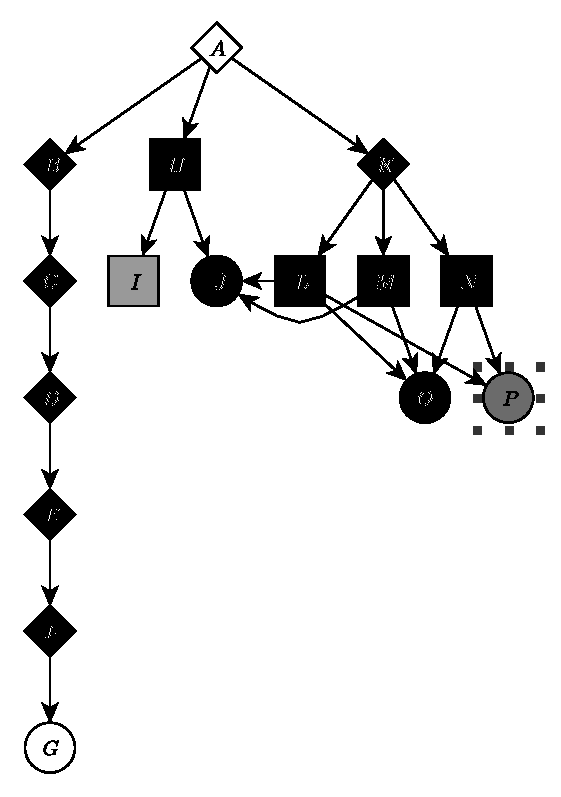
\includegraphics[scale=1.0]{images/trust-beispiel.pdf}
  \caption{Beispiel für die Berechnung der Gültigkeit von Schlüsseln}
  \label{fig:trust-beispiel}
\end{figure}

Abbildung \ref{fig:trust-beispiel} gibt ein Beispiel für die
Berechnung der Schlüsselgültigkeit unter Verwendung der
Standard-Parameter $N=1$, $M=3$ und $L=5$. Die Schlüssel $B, H$ und
$K$ wurden direkt von $A$, dem Besitzer des Schlüsselrings,
unterschrieben und sind deshalb voll gültig. Da $L, M,$ und $N$ von
$K$ unterschrieben wurden und dieser über volles Vertrauen verfügt,
sind sie ebenfalls voll gültig. $O$ sowie $J$ sind voll gültig, da sie
jeweils von drei Schlüsseln mit geringfügigem Vertrauen unterschrieben
wurden. $I$ und $P$ wurden dagegen jeweils nur von zwei Schlüsseln mit
geringfügigem Vertrauen unterschrieben und sind deshalb nicht voll
sondern nur eingeschränkt gültig. $G$ wurde zwar von einem voll
gültigen Schlüssel mit vollem Vertrauen unterschrieben. Allerdings
überschreitet die Signaturkette zu $A$ die maximale Länge von 5 und
wird deshalb nicht betrachtet.

Ein öffentlicher Schlüssel, der anhand dieser Regeln nicht als
authentisch verifiziert werden kann, kann trotzdem zur Verschlüsselung
und zur Verifizierung von Signaturen verwendet werden. Allerdings
warnt GnuPG in diesem Fall vor der Verwendung.

\subsection{Zustandekommen von Signaturen im Web of Trust}
\label{sec:sozi-komp-des}

\subsubsection{\"Ubliche Zertifizierungsprozeduren}
\label{sec:ubliche-zert}

Bis jetzt wurde nur erkl\"art, dass eine Signatur die
Zusicherung \"uber die Bindung eines Schl\"ussels an eine Person,
d.h. eine Identit\"at, darstellt. In diesem Abschnitt wird n\"aher
darauf eingegangen, wie solche Zusicherungen \emph{\"ublicherweise}
zustande kommen. Ausserdem werden einige Aspekte (FIXME
Rahmenbedingungen)

Bemerkt werden muss, dass der Zertifizierungsprozess im Kontext des
Web of Trust nicht formal definiert ist. Weder der OpenPGP-RFC noch
andere Standarddokumente machen dazu Vorschriften. Nur Certificate
Authorities, die PGP verwenden, und einige wenige Privatpersonen
dokumentieren ihre Verfahren zur Zertifizierung in Form von
sogenannten ``Keysigning-Policies''. Ausserdem ist dem Autor dieser
Arbeit keine Studie \"uber tats\"achlich verwendete Mechanismen
bekannt. Deshalb wird an dieser Stelle nur anekdotische Evidenz
als Eindruck von \"ublichen Praktiken pr\"asentiert.

Die Person, die eine Signatur erstellt, wird im folgenden mit
\emph{Unterzeichner}, und die Person, deren Schl\"ussel
unterschrieben wird, mit \emph{Unterzeichneter} bezeichnet. Um
die oben erw\"ahnte Zusicherung abgeben zu k\"onnen, muss der
Unterzeichner die Identit\"at des Unterzeichneten \"uberpr\"ufen und
so sicherstellen, dass sie mit der auf dem Schl\"ussel angegebenen
Identit\"at (in Form der \emph{UserID}) \"ubereinstimmt. Diese
\"Uberpr\"ufung sollte in Form eines \emph{pers\"onlichen} Treffens
stattfinden, da sonst eine sinnvolle Identit\"ats\"uberpr\"ufung im
Allgemeinen nicht m\"oglich ist. Der Unterzeichnete sollte zuerst den
Fingerabdruck seines Schl\"ussels pr\"asentieren. Anhand dieses
Fingerabdrucks kann der Unterzeichnete \"uberpr\"ufen, dass der zu
unterschreibende Schl\"ussel tats\"achlich der des Unterzeichneten
ist.  Der Unterzeichnete sollte dann ein Dokument pr\"asentieren, dass
seine Identit\"at belegt. Um die Verwendung von gef\"alschten
Dokumenten zu erschweren, wird \"ublicherweise ein amtliches
Ausweisdokument mit Lichtbild gefordert (Personalausweis,
Reisepass). Der Unterzeichner kann nun anhand des Dokumentes
\"uberpr\"ufen, dass der Unterzeichner mit der auf dem Schl\"ussel
vermerkten Identit\"at identisch ist. Damit kann der Unterzeichner den
Schl\"ussel unterschreiben und die obige Zusicherung
abgeben. Normalerweise werden beide Teilnehmer ihre Schl\"ussel
gegenseitig unterschreiben, also die Rollen von Unterzeichner und
Unterzeichnetem wechseln.

Dies sind die \"ublichen Anforderungen an einen
Zertifizierungsprozess, wie sie von ernsthaften Benutzern des Web of
Trust erwartet werden. Allerdings hindert einen Teilnehmer nichts
daran, diese Anforderungen beliebig abzuschw\"achen. Er kann
beispielsweise auf die Identit\"ats\"uberpr\"ufung von Personen
verzichten, die ihm pers\"onlich bekannt sind oder im Extremfall auf
jegliche \"Uberpr\"ufung verzichten. Allerdings ist jeder Benutzer
selbst daf\"ur verantwortlich zu entscheiden, welchen Personen er
dahingehend vertraut, korrekte Zusicherungen abzugeben.

\subsubsection{Certificate Authorities im Web of Trust}
\label{sec:cert-auth-im}

Eine Reihe von Einrichtungen agiert im Kontext des Web of Trust als
\emph{Certificate Authorities} im Sinne von Abschnitt
\ref{ch:Grundlagen:sec:PublicKeyCrypto:subsec:KeyAuth:subsubsec:PKI}. Diese
Einrichtungen bieten als Dienstleistung die Signierung von
PGP-Schl\"usseln nach \"Uberpr\"ufung der Identit\"at an. Der Prozess
bzw. die Kriterien, nach dem diese Signaturen zustande kommen, ist
dokumentiert. Dieser Prozess unterscheidet sich \"ublicherweise nicht
von dem in Abschnitt \ref{sec:ubliche-zert} beschriebenen Vorgehen.

\begin{itemize}
\item Der Heise-Verlag betreibt seit 1997 eine Certificate Authority
  im Rahmen der ``Krypto-Kampagne''. Diese hat sich zum Ziel gesetzt,
  die Verbreitung von PGP zu f\"ordern. Durch eine kostenlose
  Certificate Authority soll das Web of Trust gest\"arkt werden (FIXME
  cite).

  Die Zertifizierung wird auf Messen gegen Vorlage des
  Personalausweises angeboten. Die von dieser CA verwendeten
  Schl\"ussel haben insgesamt ca. 22000 Signaturen erstellt.
\item Die Certificate Authority CACert (FIXME link) zertifizert unter
  anderem auch OpenPGP-Schl\"ussel. Der von dieser CA verwendete
  Schl\"ussel hat ca. 3400 Schl\"ussel signiert.
\item Das Deutsche Forschungsnetzwerk (DFN) betrieb vermutlich bis zum
  Jahr 2009 eine Certificate Authority f\"ur PGP.
\end{itemize}

Das Konzept einer Certificate Authority steht nicht grunds\"atzlich im
Widerspruch zu einem Web of Trust. Eine Verifizierungsprozedur wie in
Abschnitt \ref{sec:ubliche-zert} macht f\"ur einen Schl\"ussel einer
Certificate Authority keinen Sinn, da er \"ublicherweise nicht mit
einer einzelnen Person verbunden ist. Ein Benutzer muss sicherstellen,
dass der CA-Schl\"ussel authentisch ist und entscheiden, ob er dem
Betreiber dahingehend vertraut, die dokumentierte Policy FIXME
zuverl\"assig umzusetzen. Zus\"atzlich muss allerdings der
CA-Schl\"ussel signiert werden, um seine Signaturen benutzen zu
k\"onnen. Werden diese Signaturen auf dem CA-Schl\"ussel
ver\"offentlicht, dann ergeben sich Signaturpfade, die zu diesem
Schl\"ussel f\"uhren. Der CA-Schl\"ussel kann dann auch von
Teilnehmern, die ihn nicht direkt unterschrieben haben, als Teil ganz
normaler Signaturketten verwendet werden (sofern sie dem Betreiber der
Certificate Authority vertrauen). Certificate Authorities f\"ugen sich
also problemlos in das dezentrale Web of Trust ein.

\subsubsection{Keysigning-Parties}
\label{sec:keysigning-parties}

Das in Abschnitt \ref{sec:ubliche-zert} beschriebene \"ubliche
Verfahren betrifft zun\"achst nur zwei Personen. Wenn mehrere Personen
zusammenkommen, um ihre Schl\"ussel gegenseitig zu unterschreiben,
wird von einer \emph{Keysigning-Party} gesprochen. Die Bandbreite
dieser Veranstaltungen ist sehr gross. Sie reicht von informellen
Zusammenk\"unften mehrerer Personen, die paarweise ihre Schl\"ussel
unterschreiben, bis hin zu gr\"osseren, formalisierten Veranstaltungen
im Kontext von Konferenzen und Messen. Bei gr\"osseren Veranstaltungen
wird \"ublicherweise eine Anmeldung der Teilnehmer erwartet. F\"ur
gr\"ossere Veranstaltungen hat sich eine Reihe von ``Protokollen''
etabliert, um den Ablauf effizient zu organisieren\cite{Brennen2008}.

Gr\"ossere Keysigning-Parties fanden im Jahr 2009 beispielsweise auf
diesen Veranstaltungen statt:
\begin{itemize}
\item Debconf (Konferenz des Debian-Projekts) mit XXX Teilnehmern
\item FOSDEM (Open-Source-Konferenz) mit XXX Teilnehmern
\item LinuxTag (Messe) mit XXX-Teilnehmern
\end{itemize}

Offensichtlich ist die Obergrenze der Signaturen, die aus einer
Keysigning-Party mit $n$ Teilnehmern entstehen k\"onnen, $n^2$. Schon
bei Veranstaltungen mit wenigen hundert Teilnehmern werden also
erhebliche Mengen von Signaturen dem Web of Trust hinzugef\"ugt.

Insbesondere auf kleinen und spontanen Veranstaltungen ist es jedem
Teilnehmer \"uberlassen, mit welchen anderen Teilnehmern er Signaturen
austauscht. \"Ublich ist allerdings, dass (fast) alle Paare von
Teilnehmern Signaturen austauschen. Ein hervorstechendes Merkmal
vieler Keysigning-Parties ist also eine (fast) vollst\"andige
Vernetzung ihrer Teilnehmer.


\subsubsection{Foobar FIXME}
\label{sec:foobar-fixme}

In einer Reihe von Open-Source-Projekten spielen PGP und das Web of
Trust eine wichtige Rolle. Im Debian-Projekt beispielweise werden
PGP-Schl\"ussel unter anderem benutzt, um alle bereitgestellten
Softwarepakete durch den zust\"andigen Entwickler signieren zu
lassen. Auf diese Weise wird \"uberpr\"uft, dass ein hochgeladenes
Paket tats\"achlich von dem verantwortlichen Projektmitglied stammt
und nicht ver\"andert wurde. Dazu muss jeder Debian-Entwickler \"uber
einen Schl\"ussel verf\"ugen, der von mindestens einem anderen
Debian-Entwickler verifiziert und unterschrieben wurde. Auf diese
Weise bildet sich bereits innerhalb des Projekts ein Web of Trust,
dass einen Teil des globalen Web of Trust darstellt. PGP scheint eine
wichtige Rolle in der Kultur des Projekts zu spielen. Darauf weist
beispielsweise hin, dass auf Treffen von Projektmitgliedern oft
Keysigning-Parties abgehalten werden, um das Web of Trust zu
st\"arken. Ausserdem signiert eine \"uberdurchschnittliche Anzahl von
Debian-Entwicklern ihre E-Mails auf projektinternen Mailinglisten.

\section{Graphentheorie und Netzwerkanalyse}
\label{sec:graph-und-netzw}

\subsection{Graphentheorie allgemein}
\label{ch:Grundlagen:sec:Graphentheorie}

Dieser Abschnitt f\"uhrt einige grundlegende graphentheroretische
Begriffe nach \cite{Brandes2004} ein.
  
Ein \emph{Netzwerk} bezeichnet eine Ansammlung von Objekten, zwischen
denen bilaterale Beziehungen bestehen. Das hier betrachtete Netzwerk
besteht aus einer Ansammlung von OpenPGP-Schl\"usseln, zwischen denen
Beziehungen in Form von Signaturen bestehen. Ein Netzwerk kann durch einen
Graphen repr\"asentiert werden.

Ein \emph{Graph} $G=(V, E)$ besteht aus einer endlichen Menge $V$ von
\emph{Knoten} und einer endlichen Menge $E$ von \emph{Kanten}, die je
zwei Knoten miteinander verbinden. Die Anzahl $|V|$ der Knoten wird mit
$n$ und die Anzahl der Kanten mit $m$ bezeichnet. Zwei durch eine
Kante verbundene, \emph{benachbarte} Knoten heissen
\emph{adjazent}. In einem \emph{ungerichteten} Graphen ist $E$ eine
Teilmenge von $V\times V$, also eine Menge von Kanten $\{u, v\}$, die
zwei Knoten $u \in V$ und $v\in V$ verbinden. In einem
\emph{gerichteten} Graphen besteht eine Kante aus einem geordneten
Paar $(u, v)$ von Knoten. Eine gerichtete Kante $(u, v)$ f\"uhrt vom
\emph{Ursprung} $u$ zum \emph{Ziel} $v$.

Ein Graph ist \emph{vollst\"andig}, wenn er alle m\"oglichen Kanten
enth\"alt.

Der \emph{Grad} $d(v)$ eines Knotens $v$ in einem ungerichteten
Graphen bezeichnet die Anzahl der Kanten, die diesen Knoten
enthalten. Die \emph{Nachbarschaft} $N(v)$ bezeichnet die Menge der
Knoten, die zu $v$ adjazent sind. In einem gerichteten Graphen
bezeichnet der \emph{eingehende Grad} $d^{-}(v)$ die Anzahl der
Kanten, die den Knoten $v$ als Ziel enthalten, und der
\emph{ausgehende Grad} $d^{+}(v)$ die Anzahl der Kanten, die $v$ als
Ursprung enthalten.

Ein \emph{Kantenzug} zwischen Knoten $v_0$ und $v_k$ in einem Graphen
$G=(V, E)$ ist eine alternierende Folge $(v_0, e_1, v_1, e_2, \dots,
v_{k-1}, e_k, v_k)$, wobei $v_i \in V$, $e_i \in E$, sowie $e_i =
\{v_{i-1}, v_{i}\}$ in einem ungerichteten Graphen bzw. $e_i =
(v_{i-1}, v_{i})$ in einem gerichteten Graphen. Der Kantenzug hat die
\emph{L\"ange} $i$. Ein Kantenzug heisst \emph{einfach}, wenn $e_i \ne
e_j$ f\"ur $i \ne j$ gilt.  Ein einfacher Kantenzug heisst
\emph{Pfad}, wenn $v_0, \dots, v_k$ paarweise verschieden sind. Die
\emph{Distanz} $d(u, v)$ von einem Knoten $u$ zu einem Knoten $v$ ist die
L\"ange eines k\"urzesten Pfades zwischen $u$ und $v$. Besteht kein
Pfad von $u$ nach $v$, so wird $d(u,v) = \infty$ definiert.


Ein Graph $G' = (V', E')$ ist ein \emph{Teilgraph} eines Graphen $G =
(V, E)$, wenn $E' \subseteq E$ und $V' \subseteq V$ gelten. Ein
Teilgraph $G' = (V', E')$ eines Graphen $G$ ist durch eine eine
Knotenmenge $V'$ \emph{induziert}, wenn $E' = \{(u, v) : u \in V, v
\in V, (u, v) \in E\}$ gilt.

Eine Partitionierung eines Graphen bezeichnet eine Zerlegung der
Knotenmenge in disjunkte Teilmengen.

Ein ungerichteter Graph heisst \emph{zusammenh\"angend}, wenn es
zwischen allen Knotenpaaren $u, v$ einen Pfad gibt. Eine
\emph{Zusammenhangskomponente} eines Graphen $G$ ist ein
\emph{maximaler}, zusammenh\"angender induzierter Teilgraph von
$G$. Ein gerichteter Graph ist \emph{stark zusammenh\"angend}, wenn es
f\"ur jeden Knoten einen gerichteten Pfad zu jedem anderen Knoten gibt. Eine
\emph{starke Zusammenhangskomponente} eines Graphen $G$ ist dann ein
maximaler, stark zusammenh\"angender induzierter Teilgraph von $G$.

\subsection{Netzwerkstatistiken}
\label{ch:Grundlagen:sec:Netzwerkanalyse:subsec:Statistiken}

In diesem Abschnitt werden einige Kennzahlen nach
\cite{Brinkmeier2004} definiert, die die Struktur eines Graphen
charakterisieren.

Die Distanz zwischen zwei Knoten wurde bereits im vorherigen Abschnitt
definiert. Ausgehend davon k\"onnen die Distanzen \emph{eines Knotens}
durch die durchschnittliche Distanz dieses Knotens zu allen anderen
Knoten charakterisiert werden:

\begin{equation}
  \label{eq:1}
  \bar{d}(u) = \frac{1}{n-1} \sum_{v \ne u} d(u, v)
\end{equation}

F\"ur einen gesamten Graphen gibt die \emph{charakteristische oder
  durchschnittliche Distanz} den Durchschnitt aller Distanzen in
diesem Graphen an:

\begin{equation}
  \label{eq:2}
  \bar{d} = \frac{1}{n^2 - n} \sum_{u \ne v \in V} d(u, v)
\end{equation}

Die \emph{Eccentricity} eines Knotens $u$ ist definiert als die
maximale Distanz zu einem anderen Knoten, also

\begin{equation}
  \label{eq:3}
  \epsilon(u) = \max\{d(u,v) | v \in V\}
\end{equation}

Davon ausgehend  wird der \emph{Durchmesser} eines Graphen als Maximum
und der Radius als Minimum \"uber die Eccentricity aller Knoten
definiert. Durchmesser und Radius geben also die Ober-
bzw. Untergrenze der Pfadl\"ange an, mit der ein Knoten alle anderen
Knoten erreichen kann. Bemerkt werden muss, dass alle auf Distanzen
basierenden Kennzahlen im Falle eines nicht (stark)
zusammenh\"angenden Graphen unendlich sind. Dieses Problem wird im
weiteren vermieden, indem diese Kennzahlen nur f\"ur (starke)
Zusammenhangskomponenten berechnet werden.

Als Verallgemeinerung der Nachbarschaft eines Knotens wird die
\emph{h-Nachbarschaft} eines Knotens als
\begin{equation}
  \label{eq:4}
  N_h(v) = \{ u \in V | d(v, u) \le h \}
\end{equation}
definiert, d.h. die Menge der Knoten, zu denen die Distanz von $v$ aus
h\"ochstens $h$ betr\"agt.

Der \emph{Clustering-Koeffizient} nach Watts und Strogatz ist ein Mass
daf\"ur, wie \emph{transitiv} die Beziehungen in einem Netzwerk
sind. Ein hoher Clustering-Koeffizient steht f\"ur eine hohe
Wahrscheinlichkeit, dass zwei Nachbarn $v$ und $w$ eines Knotens $u$
auch untereinander verbunden sind. Sei $G = (V, E)$ ein ungerichteter
Graph. Ein Dreieck $\bigtriangleup = \{V_{\bigtriangleup},
E_{\bigtriangleup}\}$ ist ein vollst\"andiger Teilgraph der Gr\"osse 3
von $G$. Die Anzahl der Dreiecke \emph{eines Knotens} wird mit
$\lambda(v) = |\{\bigtriangleup : v \in V_{\bigtriangleup}\}|$
bezeichnet. Ein \emph{Tripel} an einem Knoten $v$ ist ein Teilgraph
von $G$ bestehend aus 2 Kanten sowie $v$ und 2 weiteren Knoten, so
dass beide Kanten $v$ enthalten. Die Anzahl der Tripel eines Knotens
$v$ kann durch den Grad $d(v)$ ausgedr\"uckt werden als
$\tau(v)=\binom{d(v)}{2}$. Der \emph{lokale} Clustering-Koeffizient
$c_v$ eines Knotens wird dann als
\begin{equation}
  \label{eq:5}
  c(v) = \frac{\lambda(v)}{\tau(v)}
\end{equation}
definiert. $c(v)$ gibt also gewissermassen an, wie viele der
m\"oglichen Dreiecke an $v$ auch tats\"achlich Dreiecke sind. Der
globale Clustering-Koeffizient von $G$ ist dann
\begin{equation}
  \label{eq:6}
  C(G) = \frac{1}{|V'|} \sum_{v \in V'}c(v)
\end{equation}
wobei $V' = \{v \in V : d(v) \ge 2\}$ gesetzt wird, um nicht
definierte Werte f\"ur $\tau(v)$ zu vermeiden.

Die \emph{Transitivity} nach Newman et al. dr\"uckt zwar den gleichen
Sachverhalt aus wie der in dieser Arbeit verwendete
Clustering-Koeffizient, ist aber nicht \"aquivalent zu diesem und
sollte nicht verwechselt werden.

\subsection{Netzwerkmodelle}
\label{sec:netzwerkmodelle}

\cite{Barabasi1999} 
baz

\subsection{Soziale Netzwerke}
\label{sec:soziale-netzwerke}

Ein \emph{soziales Netzwerk} ist nach Newman\cite{newman:167} eine
Menge von Personen bzw. Gruppen von Personen, zwischen denen
Beziehungen bzw. Kontakte bestehen. Die Art dieser Interaktionen ist
dabei beliebig: Soziale Netzwerke, die in der Literatur analysiert
wurden, beinhalten Freundschaftsnetzwerke von Schulkindern, Netzwerke
von sexuellen Kontakten und Netzwerke von Gesch\"aftsbeziehungen
(ebd.).

Die im Web of Trust vorhandenen Schl\"ussel k\"onnen als
Repr\"asentationen der Besitzer dieser Schl\"ussel gedacht
werden. Allerdings ist dies keine Eins-zu-eins-Beziehung, da eine
Person \"uber beliebig viele Schl\"ussel verf\"ugen kann. Die
Beziehung dieser Personen im Web of Trust repr\"asentiert zun\"achst
nur eine Signatur, also eine Zusicherung \"uber die Bindung zwischen
dem signierten Schl\"ussel und dem Besitzer. Es scheint allerdings
recht unwahrscheinlich, dass solche Signaturen zwischen Personen
entstehen, die sich v\"ollig unbekannt sind und in keiner Beziehung
zueinander stehen. Stattdessen wird in dieser Arbeit davon
ausgegangen, dass sich Signaturen in den meisten F\"allen anhand von
bereits bestehenden sozialen Kontakten zwischen den Besitzern der
Schl\"ussel ergeben\cite{Capkun2002}. Das Sprektum m\"oglicher Beziehungen ist dabei
nat\"urlich sehr weit und umfasst mindestens alle Gruppen von
Personen, die potentiell ein Interesse an vertraulicher und
authentifizierter E-Mail-Kommunikation haben: Es kann sich dabei um
pers\"onliche Bekanntschaften handeln, also etwa um Freunde und
Bekannte. Genauso kann sich die Beziehung auch prim\"ar durch die
Mitgliedschaft in einer gemeinsamen Gruppe oder Institution
ergeben. Denkbar sind hier zum Beispiel Beziehungen, die sich aus
Arbeitsverh\"altnissen oder einer Ausbildung ergeben, also Unternehmen
oder akademische Einrichtungen. Genausogut kann es sich aber um die
Mitgliedschaft in einem Open-Source-Projekt, einem Verein oder einer
politischen Organisation handeln. Auch Zusammenh\"ange, die nicht
\"uber eine formale Mitgliedschaft in einer festen Gruppierung
entstehen, sind m\"oglich.

Zumindest im Fall von gr\"osseren, formalen Keysigning-Parties scheint
zun\"achst nicht notwendigerweise eine Verbindung zwischen den
Teilnehmern (abgesehen von der Teilnahme selbst) zu bestehen. Es ist
aber auch der Kontext relevant, in dem die Keysigning-Party
stattfindet. Bei einer Konferenz oder Messe kann es sich um ein
Ereignis mit einer klar definierten Zielgruppe handeln, die wiederum
einer Gruppe zuordnenbar ist (z.B. im Fall der
``Debconf''-Konferenzen). Ist dies nicht m\"oglich, so handelt es sich
immerhin um eine Gruppe von Personen, die \"uber ein gemeinsames
Interessengebiet verf\"ugen (beispielsweise im Fall der
``LinuxTag''-Keysigning-Parties).

\subsection{Communities}
\label{ch:Grundlagen:sec:Netzwerkanalyse:subsec:Communities}

Dieser Abschnitt f\"uhrt den Begriff der \emph{Community} ein,
definiert das G\"utemass \emph{Modularity} und beschreibt einige
Algorithmen zur Erkennung von Communities in Netzwerken. Sofern nicht
anders angegeben, wurde als Quelle ein \"Ubersichtsartikel von
Fortunato \cite{Fortunato2010} benuzt.

\subsubsection{Grundlegende Begriffe}
\label{sec:grundl-begr}

In vielen -- insbesondere sozialen -- Netzwerken neigen die Teilnehmer
dazu, \emph{Gruppen} zu bilden. In sozialen Netzwerken bilden sich
etwa Gruppen von Teilnehmern, die \"uber famili\"are,
freundschaftliche oder professionelle Beziehungen miteinander
verbunden sind. Ein besonders intensiv untersuchter Typ solcher
Netzwerke entsteht aus Kooperations- oder Koautornetzwerken von
Wissenschaftlern, in denen sich Wissenschaftler nach ihren
Fachgebieten gruppieren. Andere Beispiele von Netzwerken, in denen
Gruppenbildung stattfindet, sind Netzwerke aus der Biologie,
beispielweise Netzwerke von Protein-Protein-Interaktionen, in denen
sich funktionell \"ahnliche Proteine gruppieren, die an den gleichen
biologischen Prozessen teilnehmen. Das hier zentrale Merkmal dieser
Gruppen oder \emph{Communities} ist die Tatsache, dass Mitglieder
einer Gruppe normalerweise deutlich mehr Beziehungen zu anderen
Mitgliedern dieser Gruppe haben als zu Teilnehmern ausserhalb. Eine
solche Community sollte sich also auch in der Struktur des Graphen
wieder finden, der das Netzwerk beschreibt. In der Tat teilen viele --
insbesondere die oben angef\"uhrten -- Beispiele von Netzwerken die
Eigenschaft, dass die Kanten des Netzwerks nicht gleichm\"assig
verteilt sind. Stattdessen finden sich Gruppen von Knoten, in denen
eine hohe Dichte von Kanten herrscht, w\"ahrend zwischen diesen
Gruppen nur wenige Kanten bestehen.

In der Literatur scheint keine strenge Definition einer Community zu
existieren, die allgemein akzeptiert ist. Stattdessen wird ein
intuitives Verst\"andis verwendet, nach dem Communities \emph{dichte}
Teilbereiche eines Graphen sind, also Gruppen von Knoten, die
untereinander ``viele'' Kanten haben, w\"arend zu nicht in der Gruppe
liegenden Knoten nur ``wenige'' Kanten bestehen.

Da ein Graph \"uber ein konkretes Netzwerk abstrahiert und nur noch
die Struktur abbildet, werden auch bei der Community-Erkennung nur
Informationen benutzt, die in der Topologie des Graphen kodiert sind. 

\cite{Girvan2002}

\subsubsection{Modularity}
\label{sec:modularity}

Eine solche hierarchische Zerlegung macht noch keine Aussage
dar\"uber, wie gut die Zerlegung auf einer bestimmten Ebene die
tats\"achliche Community-Struktur wiedergibt. Um diese Frage zu
beantworten, wurde ebenfalls von Newman als Mass f\"ur die Qualit\"at
einer Zerlegung die sogenannte \emph{Modularity} definiert. Gegeben
einen ungerichteten Graphen $G=(V, E)$ und eine Zerlegung dieses
Graphen $\mathcal{C} = C_1, ..., C_n$ wird die Modularity $Q$
definiert als
\begin{equation}
  \label{eq:modularity}
  Q =
  \frac{1}{2m}\sum_{u, v \in V}\left(A_{uv}-\frac{d_id_j}{2m}\right)\delta(C_u, C_v)
\end{equation}

\subsubsection{Weitere Algorithmen}
\label{sec:algorithmen}

Seit der Arbeit von Newman wurde eine Vielzahl weiterer Methoden zur
Erkennung von Communities vorgestellt. An dieser Stelle werden 3
Methoden n\"aher beschrieben, die in dieser Arbeit verwendet
werden. Einen Gesamt\"uberblick bietet ein \"Ubersichtsartikel von
Fortunato \cite{Fortunato2010}.

\paragraph{Algorithmus von Clauset et al.  (CNM)}
\label{sec:algor-von-girv}

\paragraph{Algorithmus von Blondel et al.}
\label{sec:algor-von-blond}

\paragraph{COPRA}
\label{sec:copra}

\paragraph{Infomap}
\label{sec:infomap}

%% ==============================
\section{Verwandte Arbeiten}
%% ==============================
\label{ch:Grundlagen:sec:RelatedWork}

\subsection{Analysen des OpenPGP-Web of Trust}
\label{ch:Grundlagen:sec:RelatedWork:subsec:wot-analysis}

An dieser Stelle wird nur auf Arbeiten eingegangen, die sich mit der
Netzwerkstruktur des Web of Trust bei PGP besch\"aftigen. F\"ur einen
\"Uberblick \"uber Arbeiten zur Struktur von anderen Netzwerken sei
auf \cite{newman:167}und f\"ur Arbeiten zur Community-Struktur von
anderen Netzwerken auf \cite{Fortunato2010} verwiesen.

Capkun et al. \cite{Capkun2002} untersuchten strukturelle Aspekte der
gr\"ossten starken Zusammenhangskomponente eines PGP-Netzwerkes aus
dem Jahr 2001. Dieses Netzwerk zeigte eine geringe charakteristische
Distanz und einen hohen Clustering-Koeffizient. Ausserdem stimmte die
Verteilung der aus- und eingehenden Grade mit einem Power-Law
\"uberein. Die Autoren argumentieren, dass Netzwerke, die aus
Zertifikatsbeziehungen entstehen, naturgem\"ass den Small-World-Effekt
zeigen, da sich die Zertifikate anhand schon bestehender
Vertrauensbeziehungen ergeben. Die Autoren geben ausserdem noch ein
Netzwerkmodell an, dass Graphen erzeugen soll, die in den
beschriebenen Charakteristiken dem PGP-Netzwerk \"ahneln.

Arenas et al. \cite{Boguna2004} analysierten ein PGP-Netzwerk aus dem
gleichen Jahr. Das Netzwerk wurde von vornherein in ein ungerichtetes
Netzwerk umgewandelt, indem nicht gegenseitige Kanten entfernt
wurden. Sie betrachteten die Gradverteilung, den
Clustering-Koeffizienten und die Korrelation von Graden benachbarter
Knoten. Dabei folgt die Verteilung der Knotengrade einem Power-Law mit
einem exponentiellen Cutoff FIXME. Der Clustering-Koeffizient des
Netzwerkes betr\"agt $C=0.4$, ist also recht hoch. Die Grade
benachbarter Knoten sind positiv korreliert. Ausserdem benutzten die
Autoren den in Abschnitt \ref{sec:grundl-begr}erw\"ahnten Algorithmus
von Girvan und Newman, um eine Community-Zerlegung des Netzwerks zu
berechnen. Die Verteilung der Gr\"osse dieser Communities folgt wieder
einem Power-Law.

Webzeugs (henning -> pgp.cs.uu.nl?, wotsap)

%%% Local Variables: 
%%% mode: latex
%%% TeX-master: "diplarb"
%%% End: 
